\documentclass[a4paper, 12pt]{article}
\usepackage{listings}
\usepackage{algpseudocode}
\usepackage{algorithm}
\usepackage{amsmath}
\usepackage{amssymb}
\usepackage{hyperref}
\usepackage{graphicx}
\graphicspath{ {images/} }


\usepackage{glossaries}


%%Color table

\usepackage{xcolor,colortbl}
\newcommand{\mc}[2]{\multicolumn{#1}{c}{#2}}
\definecolor{Gray}{gray}{0.85}
\definecolor{LightCyan}{rgb}{0.88,1,1}

\newcolumntype{a}{>{\columncolor{Gray}}c}
\newcolumntype{b}{>{\columncolor{white}}c}
%%

%%%%%%%%%%%%%%%%%%%%PYTHON CODING

% Default fixed font does not support bold face
\DeclareFixedFont{\ttb}{T1}{txtt}{bx}{n}{11} % for bold
\DeclareFixedFont{\ttm}{T1}{txtt}{m}{n}{11}  % for normal

% Custom colors
\usepackage{color}
\definecolor{deepblue}{rgb}{0,0,0.5}
\definecolor{deepred}{rgb}{0.6,0,0}
\definecolor{deepgreen}{rgb}{0,0.5,0}

% Python style for highlighting
\newcommand\pythonstyle{\lstset{
language=Python,
basicstyle=\ttm,
otherkeywords={self},             % Add keywords here
keywordstyle=\ttb\color{deepblue},
emph={MyClass,__init__},          % Custom highlighting
emphstyle=\ttb\color{deepred},    % Custom highlighting style
stringstyle=\color{deepgreen},
frame=tb,                         % Any extra options here
showstringspaces=false,           % 
basicstyle=\small,
columns=fullflexible,
}}


% Python environment
\lstnewenvironment{python}[1][]
{
\pythonstyle
\lstset{#1}
}
{}

% Python for external files
\newcommand\pythonexternal[2][]{{
\pythonstyle
\lstinputlisting[#1]{#2}}}

% Python for inline
\newcommand\pythoninline[1]{{\pythonstyle\lstinline!#1!}}
%%%%%%%%%%%%%%%%%%%%%%%%%%%%%%%%%





\title{TFM}
\author{Pilar Barbero Iriarte}
\date{\today}

\begin{document}


\maketitle

\newpage

\tableofcontents

\newpage

\mbox{}
\thispagestyle{empty}
\newpage

\pagebreak

\newpage

\section{Planteamiento del problema}

Hoy en d\'ia, muchos dispositivos cuentan con un sistema de geolocalizaci\'on GPS que nos permite conocer la localizaci\'on de un sujeto en tiempo real. Con el fin de obtener la mayor informaci\'on posible en todo momento, estas posiciones recogidas se guardan en una base de datos que puede ser temporal o permanente. En el caso de ser permanente, nos encontraremos con el problema de que la base de datos puede crecer hasta un l\'imite desmesurado en el que dispositivo que recoge y almacena esta informaci\'on llene su memoria, impidiendo almacenar posiciones nuevas. \\

En este momento, es necesario tomar la decisi\'on de borrar parte de las posiciones almacenadas, seg\'un alg\'un criterio. La dificultad en este momento es elegir el criterio con el cual eliminaremos este exceso de datos, por ejemplo, borrando posiciones repetidas o posiciones que no aporten la suficiente eficiencia en relaci\'on al espacio que ocupan en memoria. Esto introduce el concepto de funci\'on de consolidaci\'on o compactaci\'on, es decir una funci\'on que elimine un exceso de datos permiti\'endonos conservar el m\'aximo de informaci\'on posible. \\

Contamos con datos proporcionados por una empresa de telecomunicaciones de sede en Zaragoza obtenidas de una base central. Esta base recibe peri\'odicamente posiciones GPS de distintos sujetos, que inserta en una base de datos centralizada. \'Estas posiciones son tomadas por la terminal de cada operativo, almacenadas localmente en esta terminal de manera temporal y enviadas a la central en el momento de conectividad con \'esta. \\

Nos planteamos que tanto la terminal personal que lleva cada sujeto como la base centralizada pueden llegar a l\'imite no deseado, provocando que este se sature e impida la insercci\'on de nuevos datos. Con el fin de impedir esto, se va a realizar un estudio de distintas t\'ecnicas de \textit{consolidaci\'on}\ref{} con el fin de almacenar el m\'inimo de datos pero con la m\'axima informaci\'on posible.  \\

\pagebreak

\section{Datos y estructura de los datos suministrados}

Se nos suministran dos bases de datos correspondientes a dos ciudades brasile\~nas distintas, \textbf{Salvador de Bah\'ia} y \textbf{R\'io de Janeiro}. En cada de una de ellas encontramos posiciones de distintos sujetos estudiados identificados a trav\'es de un c\'odigo. Cada base de datos contiene una tabla llamada \textit{posicionesgps} en la que encontramos un registro por cada posici\'on tomada por cada sujeto entre los d\'ias 2015-02-17 08:00:05 y 2015-03-04 08:18:05. \\

La estructura de los registros es la siguiente:\\

\begin{center}
	\begin{tabular}{| l | l  |}
	\hline
	\rowcolor{LightCyan}
	\hline
  		\multicolumn{2}{|l|}{Par\'ametros} \\
	\hline
	Id & Identificador num\'erico de la posici\'on (clave primaria) \\
	IdServidor & Identificador num\'erico del servidor que realiza la inserci\'on (PK) \\
	Recurso & Nombre del recurso (tetra:1234567) \\
	Latitud & Real que representa la latitud GPS \\
	Longitud & Real que representa la longitud GPS \\
		Velocidad & Entero que representa la velocidad instant\'anea \\
	Orientaci\'on & Entero que representa la orientaci\'on respecto al norte en grados \\
	Cobertura & Booleano que indica si hay cobertura \\
	Error & Booleano que nos indica si ha habido alg\'un error en la toma de la posici\'on \\
	\hline
	\end{tabular}

\end{center}

\smallskip

En base de datos, el tipo de datos guardado es:

\begin{lstlisting}[language=bash]
mysql> explain posicionesgps;
\end{lstlisting}


\begin{center}
	\begin{tabular}{|l|l|l|l|l|}
	\rowcolor{LightCyan}
	\hline
	Field & Type & Null & Key & Default \\
	\hline
	id & bigint(10) & NO &  PRI & 0  \\
	idServidor & int(10) unsigned & NO & PRI & 0 \\
	recurso & varchar(100) & YES & MUL & NULL  \\
	latitud & double & YES & & NULL  \\
	longitud & double & YES & & NULL  \\
	velocidad & tinyint(10) unsigned & YES & & NULL  \\
	orientacion & smallint(10) unsigned & YES  & & NULL  \\
	cobertura & tinyint(10) unsigned & YES  & & NULL \\
	error & tinyint(10) unsigned  & YES & & NULL  \\
	antigua & tinyint(10) unsigned & YES  & & 0  \\
	fecha\_timestamp & timestamp & NO & MUL & CURRENT\_TIMESTAMP \\
	autom\'atico & tiniyint(10) unsigned & NO & MUL & 0  \\
	\hline
	\end{tabular}
\end{center}

\smallskip


Para este estudio se ha trabajado s\'olo con los siguientes datos,\\

\begin{enumerate}
\item Id
\item Recurso
\item Latitud
\item Longitud
\item Velocidad
\item Fecha
\end{enumerate}


\pagebreak
\subsection{An\'alisis de los datos}

\pagebreak
\subsection{Espacio en disco}

Con la cantidad de posiciones suministradas, cu\'anto ocupa cada posici\'on en disco, para hacernos una idea de cu\'antas posiciones ser\'ia posible acumular en funci\'on de la frecuencia de \'estas sobre un espacio en disco finito.

En nuestra base de datos llamada \textbf{R\'io de Janeiro} contamos con \textbf{6928467} posiciones y en \textbf{Salvador de Bah\'ia} contamos con \textbf{4599974} posiciones.

El tama\~no en disco de nuestras bases de datos es,

\begin{lstlisting}[language=bash, basicstyle=\small]
mysql> SELECT table_schema as `Database`, 
	   table_name AS `Table`,  
	   round(((data_length + index_length) / 1024 / 1024), 2) 
	   FROM information_schema.TABLES  
	   ORDER BY (data_length + index_length) DESC;

\end{lstlisting}

\begin{center}

	\begin{tabular}{| l | l | l | l |}
	\hline
	Database & Table & Size in MB & Size in KB \\
	\hline
	rio & posicionesgps & 1205.64 & 120564000 \\
	bahia & posicionesgps & 961.42 & 96142000 \\
	\hline
	\end{tabular}
\end{center}

Lo cual nos da una idea de cu\'anto puede ocupar una toma de posici\'on en disco.\\

El total de posiciones almacenadas en r\'io es de $6928467$ luego podemos estimar el tama\~no de una posici\'on en, \\
$$\frac{120564000}{6928467} = 17.4012519653 KB$$

El total de posiciones almacenadas en bah\'ia es de $4599974$, luego\\
$$\frac{96142000}{4599974} = 20.9005529162 KB$$

Podemos aproximar el tama\~no de una posici\'on por unos $19$ KB. \\

Supongamos que una consola tiene unos $1$GB de almacenamiento. Podemos almacenar unas $52631$ posiciones en estos 30GB. 

Los datos han sido recogidos entre las fechas 2015-02-17 08:00:05 y 2015-03-04 08:18:05, lo que hace una diferencia de 360 horas.

Tenemos 5014 distintos tipos de sujetos a estudiar en la base de datos de r\'io:

\begin{lstlisting}
mysql> USE rio;
mysql> SELECT COUNT(distinct(recurso)) 
	   FROM posicionesgps;
\end{lstlisting}

\begin{center}
 \begin{tabular}{|l|}
 \hline
	count(distinct(recurso)) \\
 \hline
	5014 \\
 \hline
 
 \end{tabular}
\end{center}


Lo que nos da una frecuencia de toma de :

$$ \frac{6928467}{5014 \cdot 360} = 3.83$$ posiciones a la hora.

Si aument\'aramos esta frecuencia a una posici\'on cada 30 segundos, conseguri\r'iamos una frecuencia de 120 posiciones a la hora, luego un \'unico sujeto, en una jornada laboral de 8 horas, ocupar\'ia en espacio de 19.2 MB. 

\subsection{Implementaci\'on de los datos en clases de Python}\label{sec:positionClass}

La estructura de los datos es implementable en diversos lenguajes, pero se elige Python por su simplicidad y ya que es el lenguaje cient\'ifico m\'as usado hoy en d\'ia.

Se define la clase \texttt{Posici\'on} de la siguiente manera,

\begin{python}
class Position:
    def __init__(self, id, resource, lat
    		    , lon, speed, track, date):
        self.id = id
        self.resource = resource
        self.lat = lat
        self.lon = lon
        self.speed = speed
        self.track = track
        self.date = date
\end{python}

A partir de esta clase definiremos una serie de m\'etodos propios a \'esta que nos permitir\'an saber si un punto est\'a en un vecindario asociado a la posici\'on. Vamos a utilizar la noci\'on de distancia eucl\'idea como concepto en el que apoyarnos.\\

\begin{python}
        def distance_eu(self, q):
                return math.sqrt((self.lat - q.lat)**2 
                	+ (self.lon - q.lon)**2)
\end{python}


\pagebreak
\section{Nociones de vecindario}

Con el fin de realizar los algoritmos de consolidaci\'on, hemos realizado un estudio acerca de distintos tipos de vecindarios a utilizar para los algoritmos de consolidaci\'on propios y los algoritmos de \textit{clustering} utilizados que usaremos m\'as adelante.

\subsection{Vecindario simple}

Utilizando la distancia eucl\'idea, definimos un vecindario como aquel conjunto de puntos que se  encuentran a una distancia eucl\'idea menor que $\epsilon$ con respecto su centro $p_0$, es decir,

$$ d_E(p_0, p) = \sqrt{lat_{p} - lat_{p_0})^2 + (long_{p} - long_{p_0})^2 } < \epsilon $$

donde $p$ es un punto con latitud $lat_{p}$ y longitud $long_{p}$.

Su implementaci\'on en Python es la siguiente,

\begin{python}
        def IsInneighborhoodByEUSimple(self, q, eps):
                return self.distance_eu(q) < eps
\end{python}


\subsection{Vecindario involucrando el m\'odulo de la velocidad}

En el momento que se toma la posici\'on $p_0$, aparte de la latidud y su longitud, se toma la velocidad instant\'anea del sujeto. Podemos considerar en este caso que, dado que nuestro sujeto se  encuentra a mayor velocidad, puntos m\'as alejados de lo que considerar\'iamos en el primer caso (fuera de nuestro vecindario simple), podr\'ian estar dentro de nuestro nuevo radio, que depender\'ia de la velocidad instant\'anea. As\'i, definimos nuestro nuevo vecindario:

$$ d_E(p_0, p) = \sqrt{lat_{p} - lat_{p_0})^2 + (long_{p} - long_{p_0})^2 } < \epsilon \cdot vel_{p_0} $$

donde $vel_{p_0}$ es la velocidad instant\'anea de nuestro punto centro.


Su implementaci\'on en Python es la siguiente,

\begin{python}
        def IsInNeighborhoodT0Reachable(self, q, eps):
                return self.distance_eu(q) < eps * self.speed
\end{python}


%\subsection{Vecindario involucrando el m\'odulo de la velocidad y la orientaci\'on}
%
%Igual que contamos con la velocidad instant\'anea del sujeto, contamos tambi\'en con el dato de la orientaci\'on respecto al norte de nuestro sujeto muestreado. Esta medida est\'a tomada en grados sexagesimales en el sentido de las agujas del reloj respecto al norte.
%
%Gracias a este dato, podemos calcular el vector direcci\'on que contiene la informaci\'on de la orientaci\'on de nuestro sujeto y como tambi\'en conocemos el m\'odulo de la velocidad, obtener el vector velocidad. 
%
%Nuestra componente $x$ que identificaremos con el eje del vector direcci\'on ser\'a el coseno de nuestra orientaci\'on,
%
%$$ cos(or_{p_0})$$
%
%Y nuestra componente $y$ del vector direcci\'on ser\'a el seno de nuestra orientaci\'on,
%
%$$ sin(or_{p_0}) $$

\subsection{Vecindad t0-alcanzable}

Si fijamos un intervalo de tiempo $t_0$, podemos definir una vecindad $t_0$-alcanzable como aquellos puntos que nuestro sujeto puede alcanzar en un tiempo $t_0$. Un sujeto que se desplace a velocidad reducida, tendr\'a una vecindad $t_0$-alcanzable m\'as reducido  que otro que se desplace a una velo$vel_{p_0}\cdot t_0$. 

$$ d_E(p_0, p) = \sqrt{lat_{p} - lat_{p_0})^2 + (long_{p} - long_{p_0})^2 } < vel_{p_0} \cdot t_0 $$

\'Este es un caso concreto del vecindario involucrando la velocidad. 


Su implementaci\'on en Python es la siguiente,

\begin{python}
        def is_in_neighborhoodT0Reachable(self, q, t0):
                return self.distance_eu(q) < t0 * self.speed
\end{python}

\subsection{Vecindario involucrando el tiempo}

Las posiciones de nuestros sujetos vienen muestreadas adem\'as con el instante en el que fueron tomadas. Podemos considerar que el tiempo entre tomas tambi\'en es una distancia y definir un vecindario. Definimos esta distancia temporal como la resta de ambos instantes, y el vecindario como:

$$ d_T(p_0, p) = time_p - time_{p_0} < \delta $$

\begin{python}
	def is_neighboorhoudByTime(self, q, lapse):
		foo = time.mktime(self.date.timetuple())
		bar = time.mktime(q.date.timetuple())
		return abs(foo - bar) < lapse
\end{python}


\pagebreak
\subsection{Preprocesado de datos}
Antes de empezar a realizar un algoritmo que nos realice una consolidaci\'on de los datos, es conveniente realizar un preprocesado de \'estos. \\

Un primer procesado consistir\'ia en la eliminaci\'on de todos aquellos registros que tienen como latitud y longitud $0$ ya que son datos tomados por error que lo \'unico que har\'ian ser\'ia conseguir un cl\'uster centrado en $(latitud = 0, longitud = 0)$ \\

Vamos a fijar una cantidad m\'inima de distancia, un $\varepsilon_0$, y compararemos una posici\'on con la \'ultima le\'ida para decidir si la insertamos en base de datos o no. Si la distancia del nuevo muestreo con la \'ultima es menor que este $\varepsilon_0$ fijado, desecharemos esta nueva posici\'on. Esto permite que m\'as adelante nuestro algoritmo de consolidaci\'on sea mucho m\'as r\'apido. \\


\pagebreak
\section{Algoritmos de consolidaci\'on simples}

Utilizando las nociones de vecindario definidas en la secci\'on anterior, nos planteamos la idea de definir unos algoritmos de consolidaci\'on simples con el fin de mantener la base de datos en un tama\~no m\'as o menos estable. \\

Una primera aproximaci\'on ser\'ia una creaci\'on de un trigger o un peque\~no programa en el momento de insercci\'on en base de datos que comparara la \'ultima posici\'on recibida para ese sujeto con la nueva a insertar. Se comparar\'ia la distancia entre \'estas con una distancia eucl\'idea simple, y si \'esta estuviera bajo el l\'imite permitido (es decir, muy pr\'oxima), se obviar\'ia. \\

Una segunda aproximaci\'on ser\'a definir una tarea programada \texttt{cron} (ya que nuestros dispositivos est\'an basados en una distribuci\'on de Linux) que cada cierto tiempo ejecutara una consolidaci\'on sobre estos. \\

Estas consolidaciones menos avanzadas se realizar\'an sobre posiciones antiguas, es decir, seg\'un el tama\~no de la base de datos y el nivel cr\'itico al que puede llegar a estar, mandaremos un cierto n\'umero de posiciones a realizar la consolidaci\'on. \\

\subsection{Consolidaci\'on por distancia}

Utilizando los tres tipos de vecindarios que hemos definido, definimos el siguiente m\'etodo que realizar\'a la consolidaci\'on del tipo que le indiquemos, \\


\pagebreak

\begin{algorithm}[h]\label{consolidationByDistance}
\begin{algorithmic}[1]
\Function{ConsolidationByDistance}{$positions, typeOfDistance, eps, t0$}
\For{\textbf{each} pos \textbf{in} positions}
    \If{$typeOfDistance == 'distanceEUSimple'$}
        \If{$pos.IsInNeighBorhood(next(pos), eps)$}
        	\State{Remove position in DB}
        \Else
        	\State{Maintain position in DB}
        \EndIf
    \EndIf
    \If{$typeOfDistance == 'Distance EU relative to speed'$}
        \If{$pos.IsInNeighBorhoodForEURelativeSpeed(next(pos), eps)$}
        	\State{Remove position in DB}
        \Else
        	\State{Maintain position in DB}
        \EndIf
    \EndIf
    \If{$typeOfDistance == 't0 reachable'$}
        \If{$pos.IsInNeighBorhoodForT0Reachablee(next(pos), t0)$}
        	\State{Remove position in DB}
        \Else
        	\State{Maintain position in DB}
        \EndIf
    \EndIf
\EndFor
\EndFunction
\end{algorithmic}
\caption{\label{alg:consolidationByDinstace} Algoritmo de consolidaci\'on simple por distancia}
\end{algorithm}


\subsection{Consolidaci\'on cada cierto n\'umero de posiciones}

Se puede dar el caso que la consolidaci\'on por distancia no sea lo suficientemente eficaz y no de los resultados necesarios de liberaci\'on de espacio, ya que las posiciones est\'en muy lejos entre s\'i. Como \'ulima opci\'on, se puede recurrir a un tipo de consolidaci\'on en la cual dada una lista de posiciones normalmente antiguas, se elimine un subconjunto de estas, por ejemplo, 3 de cada 5. As\'i asegurar\'iamos una p\'erdida m\'inima de informaci\'on. \\

\begin{algorithm}[h]\label{consolidationByEachSomeNumber}
\begin{algorithmic}[1]
\Function{ConsolidationByEachJinK}{$positions, j, k$}\Comment{$j < k$}
	\For{\textbf{each} pos in positions}
		\If{$position.Index \% k == 0$}
			\For{$i = 0; i < k; i++$}
				\State{Remove position with index == position.Index}
			\EndFor
		\EndIf
	\EndFor
\EndFunction
\end{algorithmic}
\caption{\label{alg:consolidationByEach} Algoritmo de consolidaci\'on cada cierto n\'umero}
\end{algorithm}


\pagebreak
\section{Algoritmos de consolidaci\'on asociados a m\'etodos de clustering}



En la secci\'on \ref{sec:positionClass} hemos definido una implementaci\'on en Python para el concepto de posici\'on. Si queremos utilizar m\'etodos de cl\'ustering m\'as avanzados, se ha de definir el concepto de \textit{cl\'uster}. \\

Definimos un cl\'uster de posiciones como un conjunto de posiciones agrupado en torno a una posici\'on singular, llamada posici\'on central del cl\'uster.\\

Realizando una sencilla implementaci\'on en Python,


\begin{python}
class Cluster:
	"Cluster of points"
	def __init__(self, center, points):
    	self.center = center
		self.points = points
\end{python}


\pagebreak
\subsection{K-means}

\textbf{K-means} es un m\'etodo eficiente de \textit{clustering} que tiene como objetivo la partici\'on de un conjunto de $n$ elementos en $k$ grupos distintos. Dado un cojunto de datos $(x_1, x_2, \ldots , x_n)$, $K-$means construye una partici\'on de las observaciones en $k$ conjuntos con $k\leq n$, $S=\{S_1, S_2, \ldots, S_k\}$ con el fin de minimizar el t\'ermino de error que es la suma de las distancias al cuadrado de cada punto al centro de su cl\'uster, es decir,

$$ E=\sum_{i=1}^{n} \sum_{x\in S_i} d(x, m_i) $$

donde $m_i$ es el centro de cada cl\'uster $S_i$ y $d(x, m_i)$ es la distancia definida entre el punto $x$ y $m_i$.

Inicialmente, el algoritmo asigna cada punto a su cl\'uster de manera aleatoria. Posteriormente, itera sobre cada punto, encuentra el centro de cl\'uster m\'as cercano y asigna el punto al cl\'uster cuyo centro est\'a m\'as cercano. Esa iteraci\'on se repite hasta que el error es peque\~no o se estabiliza.

Este algoritmo, aunque eficiente, tiene algunos inconvenientes con respecto a la consolidaci\'on de datos que se busca.
\\

La primera de todas, es que se debe fijar un n\'umero de cl\'usters a obtener desde el principio, lo que a priori no ser\'ia malo en nuestro caso, no es interesante en t\'erminos de eficiencia y de mantener la m\'axima informaci\'on posible. En todo caso, $K-$means ser\'ia interesante para un primer procesado de datos en el cual la base de datos necesitara urgentemente un descenso de cantidad de posiciones almacenadas. \\

En segundo caso, no hay distintos ente puntos considerados "ruido", ya que todos los puntos se consideran en los cl\'usters resultado. Esto introducir\'ia muchos errores a la hora de intentar minimizar el t\'ermino del error, ya que f\'acilmente se podr\'ian etiquetar posiciones no significativas como ruido y no introducirlas en el proceso.\\

Adem\'as, $K-$means es un algoritmo no determin\'istico, debido a la primera fase de asignaci\'on de centros de cl\'usters de manera aleatoria, por lo que no ser\'ia muy fiable.

\subsubsection{Estudio con Weka}

%%%%%%%%%%%%%%%%%%%%%%%%%%%%%%%%%%%%%%%%%%%%%%%%%%%%%%
TODO: Introducir estudio con Weka
%%%%%%%%%%%%%%%%%%%%%%%%%%%%%%%%%%%%%%%%%%%%%%%%%%%%%%
\pagebreak
\subsection{DBSCAN}

\textbf{DBSCAN} o \textbf{Density-based spatial clustering of applications with noise} es un algoritmo de \textit{clustering} que dado un conjunto de puntos en un espacio, los agrupa en funci\'on de la densidad de puntos que tengan a su alrededor, dejando a un lado aquellos que tienen una densidad baja. \\

Se considera un conjunto de puntos a aplicar la t\'ecnica. El algoritmo clasificar\'a los puntos en tres grupos, 

\begin{itemize}
	\item Un punto $p$ es considerado \textit{n\'ucleo} si al menos un n\'umero de puntos m\'inimo (al que denotaremos por $minPts$ est\'an a una distancia menor que $\varepsilon$ de $p$. Este conjunto de puntos se considerar\'an \textit{directamente alcanzables} desde $p$.
	\item Un punto $q$ es considerado \textit{alcanzable} de $p$ si existe un camino $p_1, \ldots, p_n$ tal que $p_1=p$ y $p_n=q$, donde cada $p_{i+1}$ es directamente alcanzable desde $p_i$ (todos los puntos del camino son puntos n\'ucleo, excepto quiz\'as $q$).
	\item Todos los puntos que no son considerados ni n\'ucleos ni alcanzables son considerados \textit{aislados}.
\end{itemize}

Ahora, si $p$ es un punto n\'ucleo, entonces forma un cl\'uster con aquellos puntos que sean alcanzables desde $p$. Cada cl\'uster contiene al menos un punto n\'ucleo; y puntos no n\'ucleo pueden formar parte de \'este, pero formaran lo que parten del \textit{borde}, ya que no permiten \textit{alcanzar} m\'as puntos. \\

\begin{figure}\label{fig:DBSCAN}
	\centering
	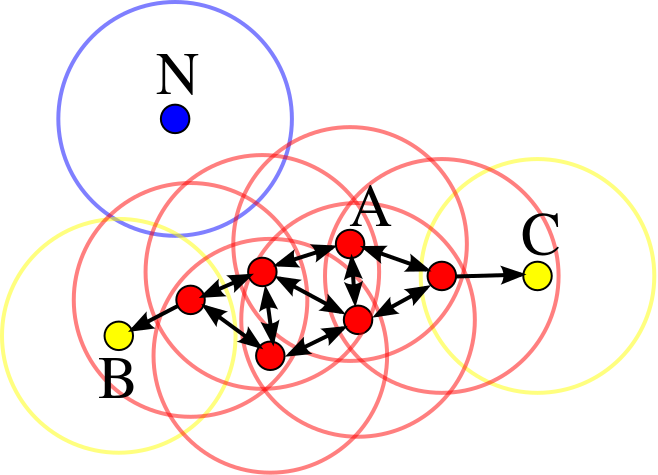
\includegraphics[scale=.5]{DBSCAN.png}
\caption{Diagrama DBSCAN}
\end{figure}

En el diagrama, se puede observar que si fijamos la variable $minPts$ a 3, el punto $A$ y los dem\'as puntos rojos son puntos n\'ucleo, ya que al menos est\'an rodeados de $3$ puntos en su vecindario de radio $\varepsilon$. Como son densamente alcanzables unos con otros, forman un cl\'uster. Los puntos $B$ y $C$ no son puntos n\'ucleo, pero s\'i que son alcanzables desde $A$, por lo que tambi\'en pertenecen al cl\'uster. El punto $N$ es calificiado como aislado o \textit{ruido} ya que no es ni punto n\'ucleo ni densamente alcanzable. \\

La alcanzabilidad no es una relaci\'on sim\'etrica ya que, por definici\'on, ningu\'un punto puede ser alcanzable por un punto no n\'ucleo (un punto no n\'ucleo puede ser alcanzable, pero no puedo \textit{"alcanzar"}). Es necesario definir una noci\'on m\'as fuerte de \textit{conectividad}. Decimos que $p$ y $q$ est\'an densamente conectados si existe un punto $o$ tal que $p$ y $q$ son densamente alcanzables. Esta noci\'on de \textit{densamente conectados} s\'i que es sim\'etrica.\\

Redefinimos la noci\'on de cl\'uster que previamente hab\'iamos definido. Un cl\'uster debe satisfacer dos propiedades:\\

\begin{enumerate}
	\item Todos los puntos deben estar mutuamente \textit{densamente conectados}.
	\item Si un punto $q$ es densamente alcanzable desde un punto $p$ del cl\'uster, $q$ es parte del cl\'uster tambi\'en. 
\end{enumerate}

\textbf{DBSCAN} requiere de dos par\'ametros para empezar: $\varepsilon$ para la noci\'on de vecindario y $minPts$ para el n\'umero m\'inimo de puntos necesario para formar un cl\'uster. Se empieza tomando arbirariamente un punto del conjunto que no haya sido visitado. Se obtiene su vecindario, en el caso de que no exista, este punto se marca como ruido y se pasa al siguiente. Si no es nulo y tiene un n\'umero de puntos mayor que $minPts$, se crea un cl\'uster. \\

Si uno de los puntos del proceso resulta que es parte de un cl\'uster, su vecindario tambi\'en se a\~nade a \'este. Se reitera este proceso, ya que todos los puntos nuevos a\~nadidos del vecindario anterior, son parte del cl\'uster, luego el vecindario de cada uno es a\~nadido. Este proceso se contin\'ua hasta que se obtiene el cl\'uster densamente conectado. \\

\begin{algorithm}[!h]\label{DBSCAN}
\begin{algorithmic}[1]
\Function{DBSCAN}{$positions, eps, minPts$}
	\State{C = 0}
	\For{\textbf{each} pos in positions}
		\If{$pos$ has been visited}
			\State{Continue next position}
		\Else
			\State{Mark $pos$ as visited}
			\State{N(pos) = NeighborPts(pos, eps)}
			\If{$length(N(pos)) < MinPts$}
				\State{Mark $pos$ as noise}
			\Else
				\State{C = next Cluster}
				\State{expandCluster(pos, N(pos), C, eps, MinPts)}				
			\EndIf
		
		\EndIf
	\EndFor
\EndFunction
\State{}
\Function{expandCluster}{$P, NeighborPts, C, eps, MinPts$}
	\State{add P to cluster C}
	\For{\textbf{each} P' in NeighborPts}
		\If{P' is not visited}
			\State{Mark P' as visited}
			\State{NeighborPts' = regionQuery(P', eps)}
			\If{$length(NeighborPts') >= MinPts$}
				\State{NeighborPts = NeighborPts joined with NeighborPts'}
			\EndIf
		\EndIf
		\If{P' is not yet member of any cluster}
			\State{add P' to Cluster C}
		\EndIf
	\EndFor
\EndFunction
\State{}
\Function{NeighborPts}{$P, eps$}
	\State{return all points within P's eps-neighborhood (also P)}
\EndFunction
\end{algorithmic}
\caption{\label{alg:DBSCAN} Algoritmo DBSCAN}
\end{algorithm}


\subsubsection{Estudio con Weka}

%%%%%%%%%%%%%%%%%%%%%%%%%%%%%%%%%%%%%%%%%%%%%%%%%%%%%%
TODO: Introducir estudio con Weka
%%%%%%%%%%%%%%%%%%%%%%%%%%%%%%%%%%%%%%%%%%%%%%%%%%%%%%
\pagebreak
\subsubsection{Implementaci\'on en Python}

Podemos encontrar una implementaci\'on de \textbf{DBSCAN} en el paquete de herramientas \texttt{scikit-learn} de python\ref{scikit-learn}.\\

%%%%%%%%%%%%%%%%%%%%%%%%%%%%%%%%%%%%%%%%%%%%%%%%%%%%%%
TODO: Introducir ejemplo realizado en IPython Notebook!!
%%%%%%%%%%%%%%%%%%%%%%%%%%%%%%%%%%%%%%%%%%%%%%%%%%%%%%


\pagebreak
\subsection{DJ-Cluster}

\textbf{Density-Joinable Cl\'uster}\ref{importantPlaces} es un tipo de algoritmo de \textit{clustering} cuya realizaci\'on depende de la distancia elegida, la cual nos generar\'a un tipo de vecindario en concreto. Este algoritmo localiza puntos significativos sobre el conjunto de todos los puntos, es decir, el centro del cl\'uster. No debemos olvidar que nuestro objetivo es encontrar posiciones significativas en todo nuestro conjunto de posiciones GPS, y \'estos centros de cl\'uster que nos generar\'a este algoritmo nos servir\'an para tal prop\'osito. \\

La idea del algoritmo es la siguiente, para cada punto, calculamos su vecindario. Este vecindario depender\'a de la distancia elegida entre todas las anteriores definidas, y seg\'un cu\'al sea la elegida, depender\'a de una variable $\varepsilon$ o un instante $t_0$ escogido. Se impone la condici\'on de que el n\'umero de puntos conseguido al computar su vecindario sea al menos un \textit{MinPts} definido previamente. Si esta condici\'on no se cumple, se marca la posici\'on actual como \textit{ruido} y se prosigue con la siguiente. En el caso de cumplirse, este nuevo punto es el centro del cl\'uster, junto a su vecindario.  \\

Con este nuevo cl\'uster creado, el siguiente paso es comprobar que este cl\'uster no sea \textit{densamente acoplable} con los que ya llevamos computados. Un cl\'uster es \textit{densamente acoplable} a otro cl\'uster si existe un punto com\'un entre ambos. \\

\begin{figure}[!h]
\centering
	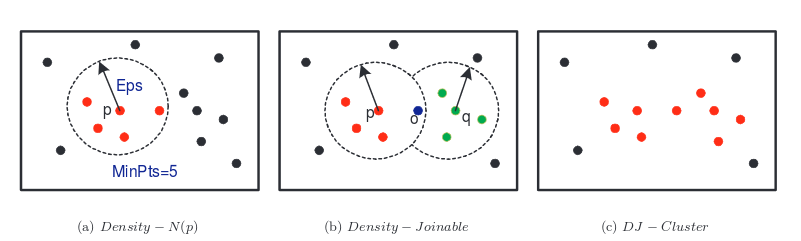
\includegraphics[scale=.7]{djcluster.png}
\caption{DJ-Clustering}
\end{figure}

\begin{algorithm}[!h]\label{djCluster}
\begin{algorithmic}[1]
	\For{\textbf{each} $p$ in set $S$}
		\State{Compute neighborhood $N(p)$ for $\varepsilon$ and $MinPts$}
		\If{$N(p)$ is null ($|N(p)| < MinPts$ for $\varepsilon$)}
			\State{Label $p$ as noise}
		\ElsIf{$N(p)$ is density-joinable to an existing cluster} 
			\State{Merge $N(p)$ with the cluster which is density-joinable}
		\Else
			\State{Create a new cluster $C$ based on $N(p)$}
		\EndIf
	\EndFor
\end{algorithmic}
\caption{\label{alg:djcluster} Algoritmo DJ-Cluster}
\end{algorithm}

Durante el proceso, se recorren todos los puntos del conjunto a analizar, calculando cada vecindario de cada punto con un centro $p$ y un radio $\varepsilon$. Si el n\'umero de puntos del vecindario excede esta cantidad m\'inima $MinPts$, entonces es un vecindario a considerar. Este cl\'uster es posteriormente \textit{mergeado} con otros posibles cl\'usters densamente acoplables. \\

Al final de cada iteraci\'on puede ser que el n\'umero de cl\'usters no cambie, porque no existe un nuevo cl\'uster o porque el nuevo cl\'uster sea mergeado con alguno de los ya existentes.\\


El valor de los par\'ametros $\varepsilon$ y $MinPts$ es el que determina el tama\~no de nuestros clusters. En nuestro caso, no buscamos grandes n\'umeros de cl\'usters, sino perder el m\'inimo de informaci\'on posible, por lo que nos convendr\'ia tomar unos valores de $\varepsilon$ y $MinPts$ peque\~nos. \ref{clusteringApproach}

El valor de la variable $\varepsilon$ debe tomarse en funci\'on de la precisi\'on de los aparatos que toman las posiciones.\ref{importantPlaces}. Podemos estimar este par\'amero por unos $20$ metros, que es la precisi\'on de un GPS convencional. \\

Con respecto al valor de $MinPts$, un valor alto de esta par\'ametro implica que los clusters deben ser m\'as densos a la hora de formarse, pero un valor razonable estar\'ia entre $3$ y $10$.\ref{clusteringApproach}.\\

La complejidad de este algoritmo es $\mathcal{O}(n\log{}n)$ \ref{importantPlaces}. \\



\subsubsection{Comparaci\'on de K-Means con DJ-Cluster}

\subsubsection{Estudio con Weka}

%%%%%%%%%%%%%%%%%%%%%%%%%%%%%%%%%%%%%%%%%%%%%%%%%%%%%%
TODO: Introducir estudio con Weka
%%%%%%%%%%%%%%%%%%%%%%%%%%%%%%%%%%%%%%%%%%%%%%%%%%%%%%
 





\pagebreak
\subsection{Canocopy}
\subsubsection{Estudio con Weka}

%%%%%%%%%%%%%%%%%%%%%%%%%%%%%%%%%%%%%%%%%%%%%%%%%%%%%%
TODO: Introducir estudio con Weka
%%%%%%%%%%%%%%%%%%%%%%%%%%%%%%%%%%%%%%%%%%%%%%%%%%%%%%

\pagebreak
\section{Conclusiones}

\pagebreak
\section{Herramientas utilizadas}

\begin{enumerate}
	\item Weka
	\item IPython Notebook
	\item R
	\item \texttt{scikit-learn}


\end{enumerate}

\newpage


\appendix
\section{Impementaci\'on de consolidaci\'on por distancia} \label{App:AppendixA}

\begin{python}
"Consolidation By distance"
def ConsolidationByDistance(listPositions, typeOfDistance, eps, t0):
	i = 0
	result = []
	while i < len(listPositions) - 1:
		# Neighborhood: Distance EU simple
		if typeOfDistance == 0:
			if not listPositions[i].is_in_neighborhoodByEUSimple(listPositions[i+1], eps):
				result.append(listPositions[i])
		# Neighborhood: Distance EU relative to speed
		elif typeOfDistance == 1:
			if not listPositions[i].is_in_neighborhoodByEURelativeSpeed(listPositions[i+1], eps):
				result.append(listPositions[i])
		# Neighborhood t0 reachable
		elif typeOfDistance == 2:
			if not listPositions[i].is_in_neighborhoodT0Reachable(listPositions[i+1], t0):
				result.append(listPositions[i])
		else:
			raise ValueError('That distance does not exist')

		i=i+1

	result.append(listPositions[len(listPositions) - 1])

	return result

\end{python}

\newpage
\section{Impementaci\'on de consolidaci\'on cada cierto n\'umero} \label{App:AppendixB}

\begin{python}
"Deletes one position every k positions."
def ConsolidationEachNumber(listPositions, k, j):
	if k >= j:
		raise ValueError('K tiene que ser menor que J')
        
	i = 0
	result = []
	while i < len(listPositions) - 1:
		if i%j == 0:
			l = 0
			while l < k:
				result.append(listPositions[i - l])
				l = l+1
			i = i+1

	return result
\end{python}


\newpage
\section{Impementaci\'on de DJ-Cluster} \label{App:AppendixC}

\begin{python}
from position import Position, Cluster

"Dj-Clustering Algorithm"
def DjCluster(setPoints, typeDistance, eps, minPoints, t0):

	listClusters = []
	listNoises = []

	for p in setPoints:
		np = computeNeighborhood(p, setPoints, typeDistance, minPoints, eps, t0)

		if np is None:
			listNoises.append(p) 
		else:
			result = np.isDensityJoinable(listClusters)

			if result is None:
				listClusters.append(np) 
			else:
				result.mergeCluster(np)

	return [listClusters, listNoises]

"Compute Neighborhood"
def computeNeighborhood(p, setPoints, typeDistance, minPoints, eps, t0):
	pointsOfCluster = []
	for q in setPoints:
		if typeDistance == 0:
			if p.is_in_neighborhoodByEUSimple(q, eps):
				pointsOfCluster.append(q)
		elif typeDistance == 1:
			if p.is_in_neighborhoodEURelativeSpeed(q, eps):
				pointsOfCluster.append(q)
		elif typeDistance == 2:
			if p.is_in_neighborhoodT0Reachable(q, t0):
				pointsOfCluster.append(q)

	if len(pointsOfCluster) < minPoints:
		return None
	else:
		return Cluster(p, pointsOfCluster)			

\end{python}

%%%%%%%%%%%%%%%%%%%%%%%%%%%%%%%%%%%%%%%%%%%%%%%%%%%%%%%%%%%%%%%%%%%%%%%%%%%%%%%%%%%%%%%%%%%%%%%%
%%%%%%%%%%%%%%%%%%%%%%%%%%%%%%%%%%%%%%%%%%%%%%%%%%%%%%%%%%%%%%%%%%%%%%%%%%%%%%%%%%%%%%%%%%%%%%%%
%%%%%%%%%%%%%%%%%%%%%%%%%%%%%%%%%%%%%%%%%%%%%%%%%%%%%%%%%%%%%%%%%%%%%%%%%%%%%%%%%%%%%%%%%%%%%%%%


\newpage

\addcontentsline{toc}{section}{Bibliograf\'ia}
\begin{thebibliography}{50}


\bibitem{lifePatter}\label{lifePatter} \textsc{Mining Individual Life Pattern} \\ \url{http://citeseerx.ist.psu.edu/viewdoc/download?doi=10.1.1.361.9085&rep=rep1&type=pdf}

\bibitem{importantPlaces}\label{importantPlaces} \textsc{Mining Personally Important Places from GPS Track} \\ \url{http://www-users.cs.umn.edu/~czhou/pub/place-important_v3.pdf}

\bibitem{clusteringApproach}\label{clusteringApproach}\textsc{Discovering Personal Gazetteers: An Interactive Clustering Approach} \\ \url{http://files.grouplens.org/papers/zhou-acmgis04.pdf}

\bibitem{scikit-learn}\label{scikit-learn} \texttt{scikit-learn} \\ \url{http://scikit-learn.org/stable/auto_examples/cluster/plot_dbscan.html} 

\end{thebibliography}



\end{document}